% CREATED BY DAVID FRISK, 2015
\chapter{Introduction}
\lettrine[findent=2pt]{\fbox{\textbf{T}}}{ }he thesis presents the study of automated visualization of the electrical system of Volvo Car Group company using data stored on the system database. The goal is to combine the artifacts found in the data together with the software metrics which are derived from analysing the needs of different stakeholders. The thesis also reports an evaluation of the provided automated visualization in the electrical department of the company. The evaluation has a purpose of determining its impact on the way of working with the Electrical Power System (EPS). 

\section{Background}\label{Background_ref}
One of the biggest challenges in automotive industry during the past few years has been to build vehicles that meet customer expectations. To overcome the challenge, more complex system of mechanical and electrical components are designed and built in modern vehicles. Besides that, a huge number of software is also integrated in order to carry out certain tasks, resulting a number of 70 of Electrical Control Unit (ECUs) deployed in a car \cite{Beeck}. For this reason, creating the architecture of the complex system is of large importance to ensure that every components and the connections between them are in the right places. \\

This thesis is done at Volvo Car Group (VCG) which is a Swedish premium automotive manufacturer that produce modern vehicles to the world. At the company, two types of architectures for electrical system are used to handle complex systems of cars \cite{Eliasson_1}. The two architectures have different abstraction levels, meaning that they serve different purposes. A high-level architecture (logical view) contains Logical Architectural Components (LAC) designed by software architects with a purpose of guiding and breakdown work to be developed during implementation phase. Development team creates a low-level architecture (design view) which represents actual structure of the electrical system. The low-level architecture also shows Logical Components (LC) which are broken down from LACs in the high-level architecture, it also shows connections between LCs, and signals they receive/send. \\

The low-level architecture is stored in a proprietary tool,  which we will call it \textit{the Database} for the rest of this report. The database stores the data such as documentations, the software components, the ECUs, the LCs, and the LACs. Using the stored data, the tool generates model shells to be implemented by software developers for in-house software development and also the tool generates requirement documents which has functionalities to be implemented by suppliers. Moreover, it can also generate ECU-integration and network communication in the electrical system \cite{Eliasson_2}.\\

When a user interacts with the Database, he/she will be presented with a complete view of the whole low-level architecture of an electrical system. The tool does not allow users to select and generate visualization of some parts of the system. The architecture is enormous which makes it difficult for the stakeholders to get what they need with less time, having experience of using the Database is quite big support in this case, meaning someone must know where to locate a needed artifact otherwise it will take a long time to get the needed information. Thus, visualization of the low-level architecture is needed. To do so, an identification of the key artifacts of electrical system must be performed since visualizing the whole architecture is unnecessary for all stakeholders. \\

\begin{figure}[H]
\centering
\captionsetup{justification=centering}
\vspace{0cm}% Adjust vertical spacing here
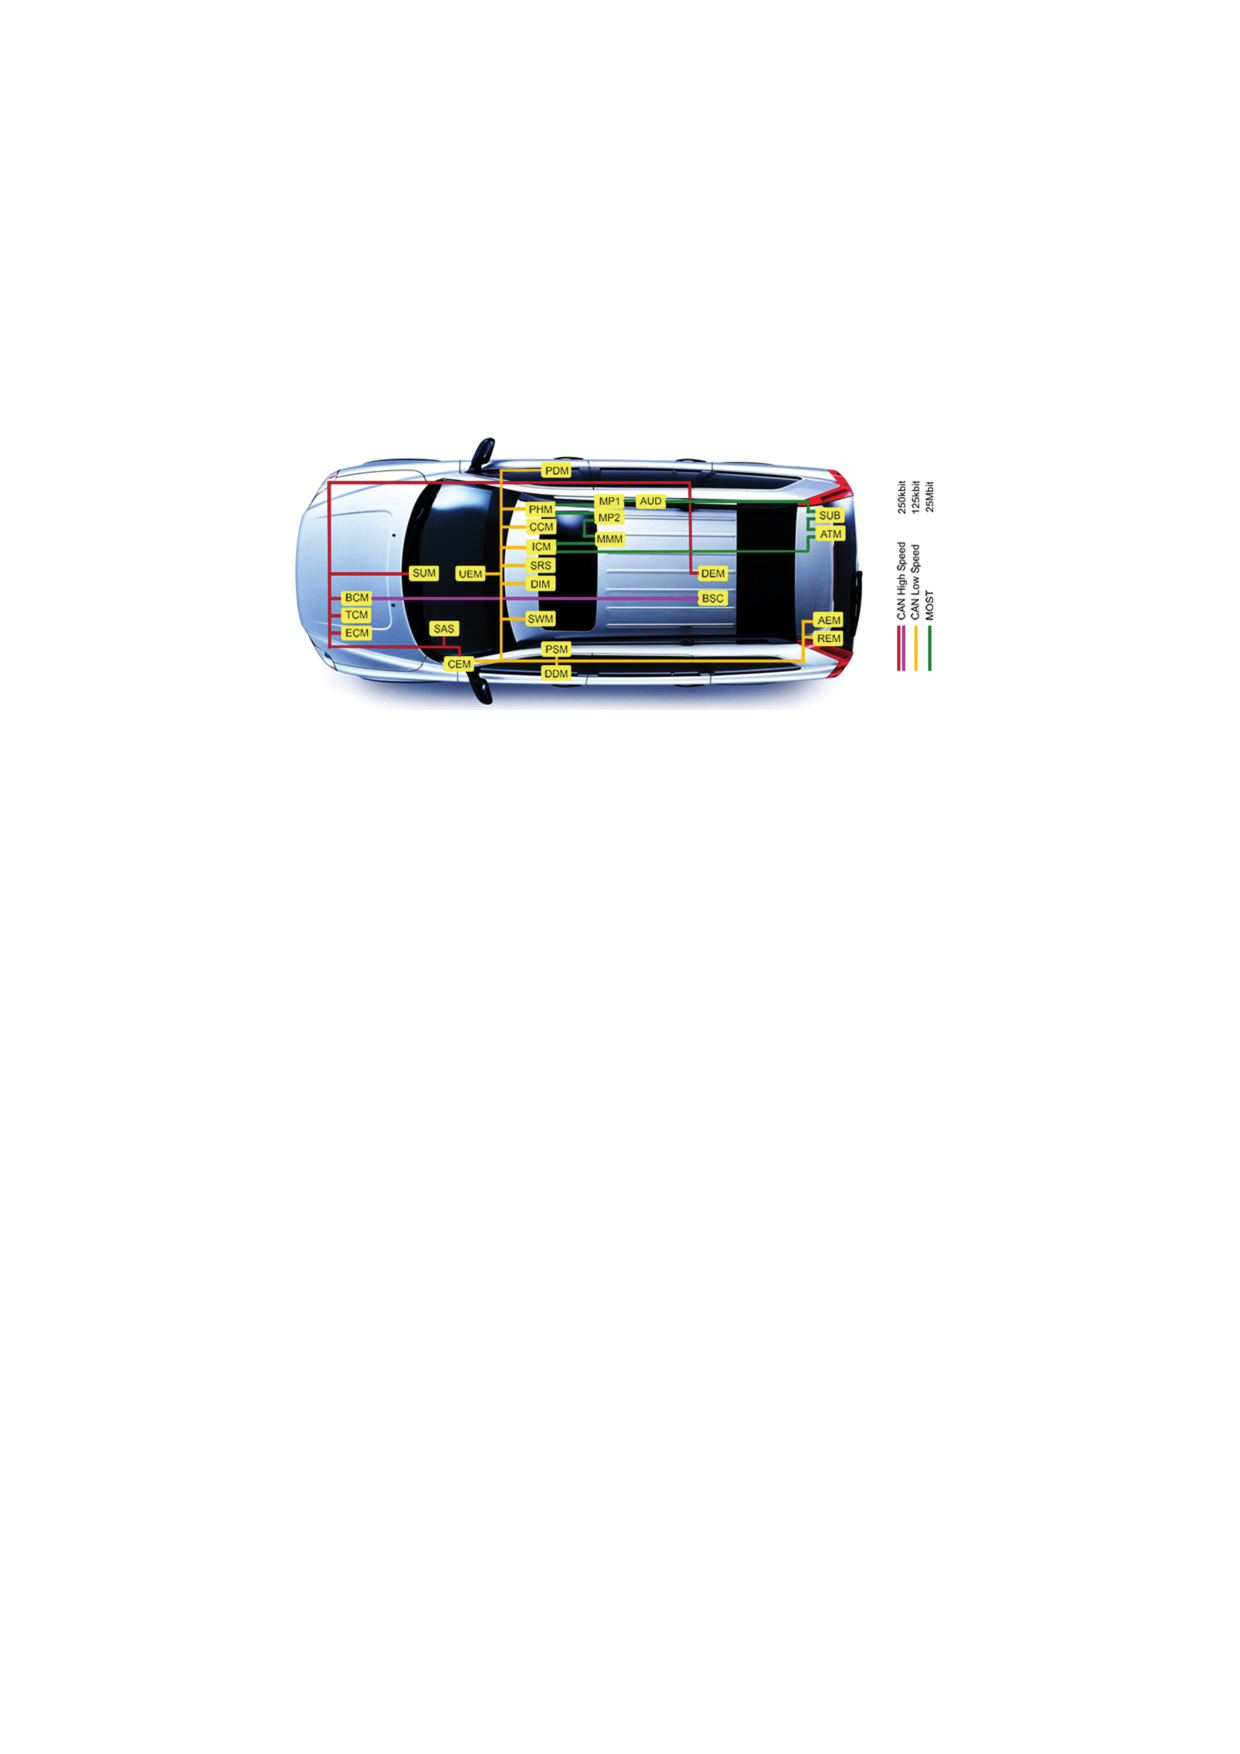
\includegraphics[width=0.9\linewidth]{figure/literatures/wallin_physical.pdf}
\caption{An example of electrical architecture of the Volvo XC90~\cite{Wallin}}
\end{figure}

Apart from what has been mentioned, there is inconsistency between the high- and the low-level architectures. The reason is that the low-level architecture is kept up-to-date by the development team during the implementation phase as the product evolves, but the high-level architecture is updated only a few times a year. Having a visualization of the low-level architecture may help to bridge the gap of inconsistency between the two levels of the architectures.


\section{Statement of the problem} \label{Statement_ref}
The first problem that this thesis work addresses is that the Database shows the irrelevant parts of the system to its users. This means, it shows the complete view which includes all components, ports, system signals, ECUs, LACs, requirements etc. Moreover, the tool does not provide a visualization. In most cases, only some parts of the data stored in the Database are relevant to the stakeholders and this depends on the individual’s interest. Due to this, it is difficult for stakeholders to locate what they are looking for unless they know where to look for it. Sometimes, the stakeholders do not even know what they are looking for and this makes a task to locate what they want even more difficult. \\

Furthermore, the diagram at VCG does not only contain the components, ports, and connections, but also a logical designs. This makes the document even bigger and harder for stakeholders to focus on only the parts that they have an interest in. \\ 

The second problem is the inconsistency between the low-level and high-level architectures. As it has been mentioned earlier, the high-level architecture gets updated few times a year, the difference arises because new features are being implemented by developers and its only the low-level architecture that gets updated instantly and so, this is the part where the inconsistency starts to occur. \\ 

To tackle these two problems, our thesis will provide a solution which helps to create automated visualization of the current architecture of the system with regard to the main interests of different stakeholders, also the solution will help high-level architects to get better understanding of what is available on the real implementation which can support a decision making.


\section{Purpose} \label{Purpose_ref}
The purpose of this thesis work is to find metrics that helps to identify the key artifacts of the electrical architecture. When visualizing a system at first, one will end up having a diagram with a lot of information. The thesis also aims to find metrics that will allow to create an optimized visualization of the electrical architecture. The metrics will be obtained from interviewing different stakeholders. This in turn will result in having different views (visualizations) of the electrical architectures with regards to the interests of stakeholders. \\


\section{Research questions} \label{IN:rq}
In order to address the problems mentioned, we have formulated two research questions. The first research question covers the identification of the needs of stakeholders towards visualization of electrical architectures and the differences among them. The second research question covers how an automated visualization helps to fulfill their needs.\\

The research questions are formulated as follows:
\vspace{0.5cm}
\begin{que} \label{que:1}
What are the needs of different stakeholders towards visualization of the electrical architectures?
\end{que}

\begin{que} \label{que:2}
How does an automated visualization fulfil the needs of stakeholders?
\end{que}


\section{Significance of the study} \label{Significance_ref}
The findings of this thesis aim to encourage the use of automated visualization, and the way of working with electrical architectures in the automotive industry. Since it has been newly introduced recently, our work will be an evidence to support the advantages of using the automated visualization. \\

For the company, the metrics that we have discovered from interviewing stakeholders and extracted data from the Database will be a powerful tool that helps to identify the important components of the architectures. On having an automated visualization, it provides an opportunity at company for further research on this area. \\

For us, as Master’s students in Software Engineering, we have had an opportunity to learn how automotive architects and stakeholders work with architectures, and understood the needs of different stakeholders. We also discovered how the automated visualization for the architectural diagrams plays an important role in an automotive domain. 

\section{Outline of the report} \label{Outline_ref}
\todo{need to be fixed}
This report is divided into 7 Chapters which can be seen in Figure~\ref{fig:report_outline}. Chapter 1 introduces the background of the thesis work, statement of the problem, the project purpose, research questions, and significance of the study. Theory related to architectures in automotive domain, software visualization, Model-driven Software Engineering, and different types of stakeholders will be discussed in Chapter 2, including the architectures at VCG and the use of the Database. Chapter 3 presents the method used in this work, which is divided into two phases. The results obtained during both phases are presented separately in Chapter 4. Chapter 5 contains the answers to the research questions presented in Section~\ref{IN:rq}. Validity threats is discussed in Chapter 6 and the last Chapter summarizes the study and what could be done in the future work.

\begin{figure}[H]
\centering
\captionsetup{justification=centering}
\vspace{0cm}% Adjust vertical spacing here
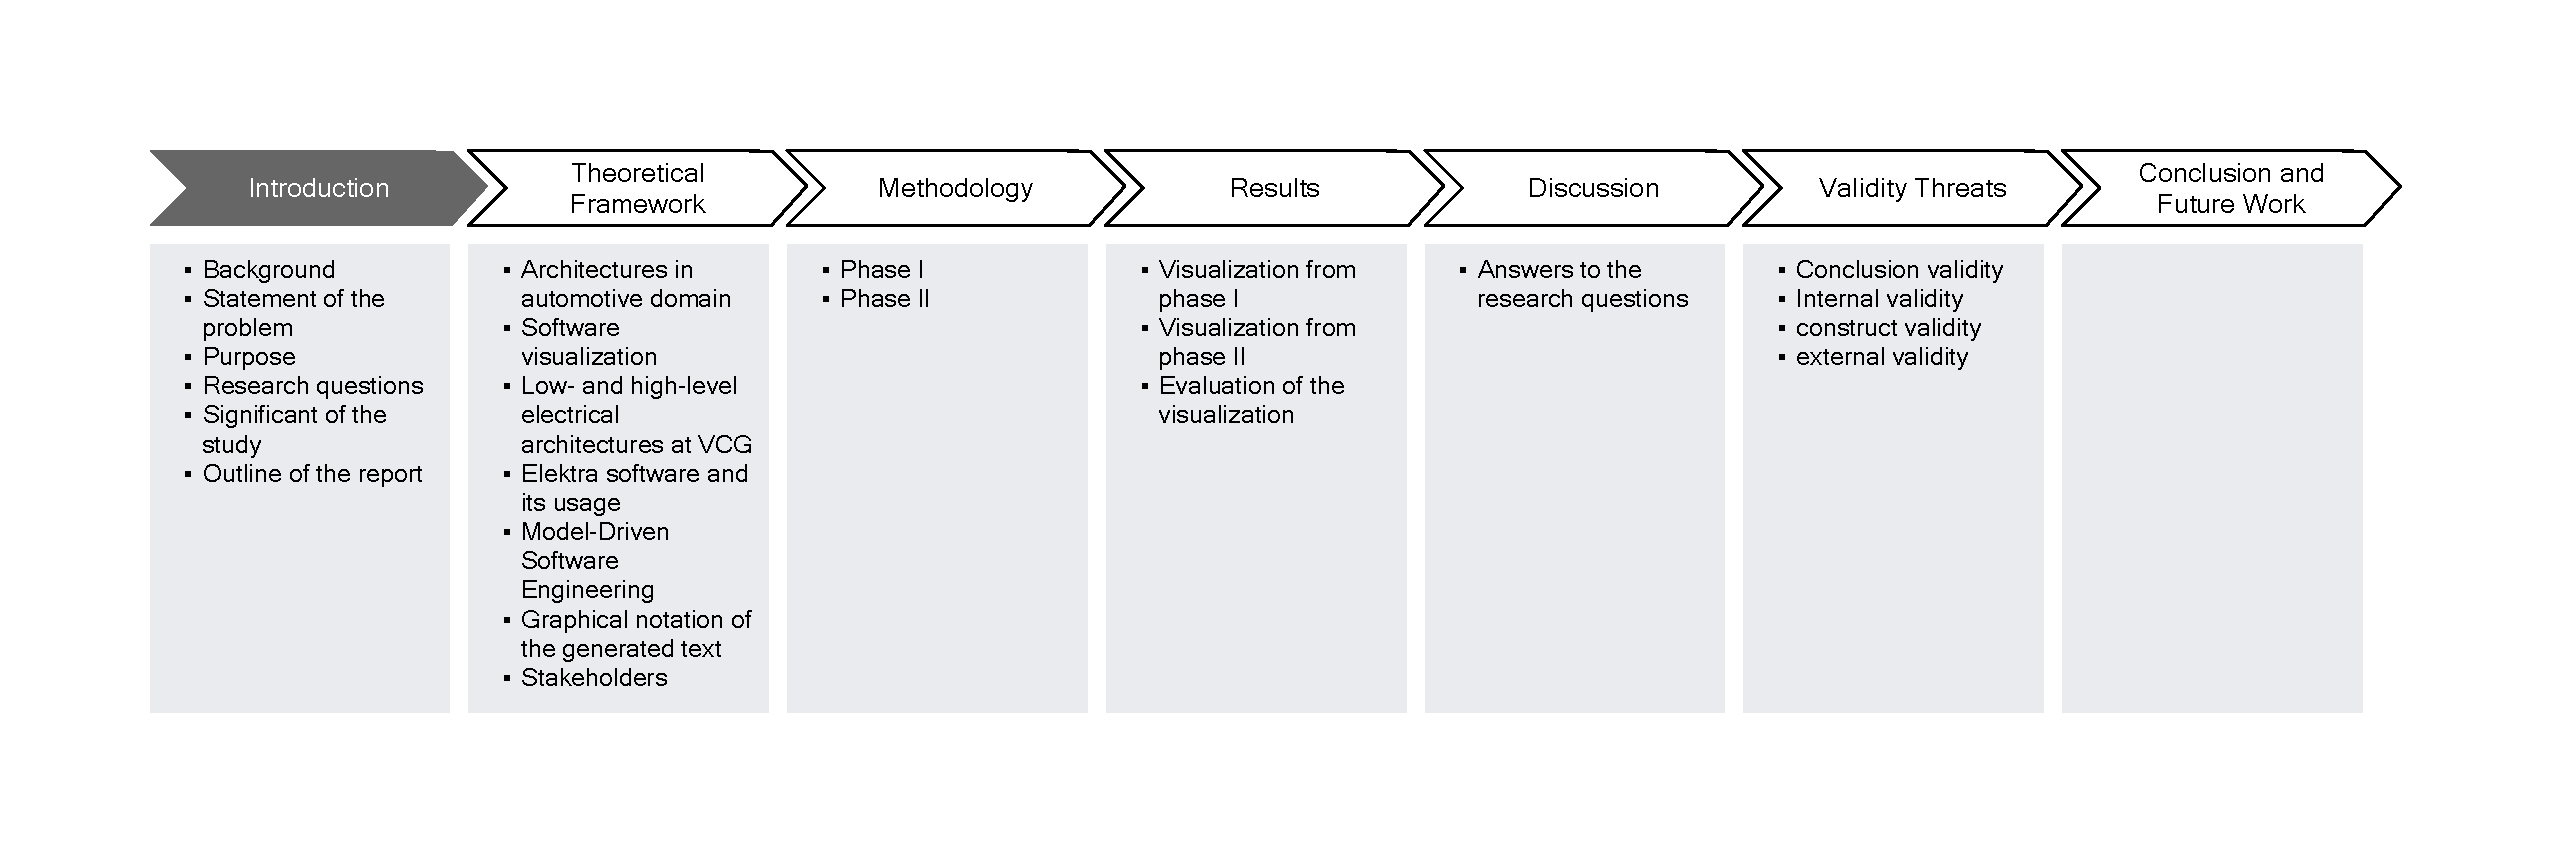
\includegraphics[width=1\linewidth]{figure/misc/report_outline.pdf}
\caption{Report outline}
\label{fig:report_outline}
\end{figure}